% The Inverse-Objective Regulator (IOR) -- system paper
% Compile with: pdflatex main && bibtex main && pdflatex main && pdflatex main
% (or latexmk -pdf main.tex). Tested against a standard TeX Live install.
%
% To switch to a conference template later, replace the documentclass and the
% geometry block with the template's class (e.g. neurips_2026.sty) and remove
% the manual geometry settings. The \input section files are template-agnostic.

\documentclass[11pt]{article}

\usepackage[utf8]{inputenc}
\usepackage[T1]{fontenc}
\usepackage[margin=1in]{geometry}
\usepackage{amsmath}
\usepackage{amssymb}
\usepackage{amsfonts}
\usepackage{booktabs}
\usepackage{tikz}
\usepackage{pgfplots}
\pgfplotsset{compat=1.18}
\usepackage{array}
\newcolumntype{P}[1]{>{\raggedright\arraybackslash}p{#1}} % ragged-right p-column
\usepackage{graphicx}
\usepackage{xcolor}
\usepackage[strings]{underscore} % lets us write sub_goal names verbatim
\usepackage{enumitem}
\usepackage{microtype}
\usepackage[numbers,sort&compress]{natbib}
\usepackage[colorlinks=true,linkcolor=black,citecolor=black,urlcolor=blue]{hyperref}

% Visible TODO marker for sections still being drafted into full prose.
\newcommand{\todo}[1]{\textcolor{red}{[TODO: #1]}}

% Placeholder box for figures whose artwork is not yet produced.
\newcommand{\figplaceholder}[1]{%
  \begin{center}
  \fbox{\parbox{0.9\linewidth}{\centering\vspace{1.5em}\textit{#1}\vspace{1.5em}}}
  \end{center}}

\title{The Inverse-Objective Regulator: Bayesian Goal Inference from\\
Agent Trajectories for Targeted Adversarial Auditing}

\author{%
  % TODO: author list and affiliations
  Aakash Sangani}

\date{}

\begin{document}
\maketitle

\begin{abstract}
Deployed artificial-intelligence agents are increasingly governed by a stated
natural-language purpose, yet no existing tool measures whether an agent actually
pursues that purpose. Agent red-teaming probes systems against fixed attack
catalogues, and inverse reinforcement learning (IRL) reconstructs an agent's
implicit objective only at the model-weight or training level, which closed
deployments do not expose. We introduce the Inverse-Objective Regulator (IOR), a
black-box system that infers a revealed objective from an agent's tool-call
trajectories using Bayesian IRL, computes its divergence from the declared
purpose over a shared feature basis, and steers adversarial probes at the
dimensions of highest divergence. A Goal Decomposition Judge bridges natural-language
purposes into the feature space IRL requires without access to model internals, and
a pluggable feature basis spans a deterministic model-free floor, a single
language-model judge, and a judge ensemble. We contribute an open gym of three
planted-divergence reference environments and report what auditing them reveals.
Divergence recovery with an Opus~4.8 judge is strong where the divergence is
expressed in observable behaviour (Pearson $r = 0.96$ on a cost-minimisation agent)
but fails where it depends on content quality the judge must assess ($r = -0.72$ on
a faithfulness agent), whereas an idealised critic recovers both ($r = 0.96$). The
method's competence is therefore bounded by the judge's reliability on the specific
sub-goals at issue rather than by the inference machinery: a column-mean ablation
shows the Bayesian IRL ranking is correlated with but not reducible to a simple
average (Spearman $0.77$), and a free-parameter sweep shows absolute scores are
tuning-dependent, so we treat the ranking of divergence dimensions, not its
magnitude, as the reportable quantity. A deterministic model-free basis predicts
held-out behaviour above a uniform baseline, establishing a reproducible floor. The
inference-probe feedback loop is presented as a design; closing it empirically, and
the targeted-probing evaluation, remain specified as protocols. Findings are
designed to map onto OWASP, MITRE ATLAS, and NIST AI RMF taxonomy nodes so that
output is legible to regulators auditing intended-purpose conformity under the EU AI
Act.

\end{abstract}

\section{Introduction}
\label{sec:intro}

The EU AI Act (Regulation 2024/1689) anchors conformity assessment on a system's
\emph{intended purpose} (Art.~9, Annex~IV)~\citep{euAIAct2024}. For deployed AI
agents, the question of whether an agent pursues its intended purpose is not
answered by capability benchmarks or static alignment tests: it requires reasoning
about what the agent is actually optimising for across sequences of real tool
calls. An agent that is told to ``find the cheapest option'' but instead maximises
the number of tool calls it makes is not failing a capability test; it is pursuing
a different objective from the one it declares.

The literature that bears on this question divides into three clusters that do not
overlap. First, agent red-teaming and misalignment benchmarks
\citep{agentMisalignment2025} probe capability and misalignment propensity using
fixed attack catalogues; they establish that deployed agents can and do behave in
misaligned ways, but they do not infer what an agent is optimising for, and they do
not use such an inference to steer probing. Second, IRL for alignment auditing
\citep{alignmentAuditor2025, ir3contrastive, insightsInverse2024} reconstructs objectives
from model weights or RLHF training signals; these methods are not applicable to
deployed black-box agents accessible only through an API. Third, goal inference
from behaviour \citep{sips2020, communicatingAgents2023} operates in structured
planning domains rather than in the unstructured tool-call space of deployed
agents.

\paragraph{The empty cell.}
No existing tool combines (a) IRL-based objective inference from tool-call
trajectories, (b) divergence computation from a declared purpose, and (c)
adversarial probe steering driven by that divergence, whilst emitting the result as
regulatory evidence. We introduce the Inverse-Objective Regulator (IOR) to occupy
this cell.

\paragraph{Contributions.}
\begin{itemize}[leftmargin=1.4em]
  \item IOR, a system design that connects goal inference to adversarial probe
  targeting at the deployed-agent level through a closed loop in which inference
  steers probing and probe results refine inference. We present the loop as a
  design and evaluate its components; closing it empirically is future work
  (Section~\ref{sec:limitations}).
  \item The Goal Decomposition Judge, which bridges natural-language declared
  purposes into the feature space that IRL requires without access to model
  weights, together with a pluggable feature basis spanning a deterministic
  model-free floor, a single judge, and a judge ensemble with quantified
  agreement.
  \item An open gym of three planted-divergence reference agents with deterministic
  seeds, enabling reproducible evaluation of objective recovery.
  \item Divergence reports mapped to OWASP ASI, MITRE ATLAS, and NIST AI RMF nodes,
  making findings directly usable in compliance workflows.
\end{itemize}

\paragraph{Scope.}
IOR operates black-box (API-level traces only, no weights or logits). It audits and
certifies; it does not enforce inline. Because IRL is ill-posed, IOR emits a
distribution over candidate objectives with uncertainty, never a single
overconfident point estimate.

\section{Background and Related Work}
\label{sec:related}

\subsection{Inverse Reinforcement Learning}
IRL recovers a reward function from demonstrated behaviour. The foundational
linear-programming formulation~\citep{ng2000algorithms} was followed by the
maximum-entropy formulation~\citep{ziebart2008maxent}, now the standard
probabilistic treatment, and by Bayesian IRL~\citep{ramachandran2007bayesian},
which places a Boltzmann likelihood over trajectories and returns a posterior over
reward weights. IOR adopts the Bayesian formulation precisely because it yields a
posterior rather than a point estimate. IRL is known to be partially identifiable:
many reward functions explain one behaviour set~\citep{partialIdentifiability2024},
which IOR addresses by reporting the full posterior.

\subsection{IRL Applied to Language-Model Alignment}
The Alignment Auditor~\citep{alignmentAuditor2025} applies Bayesian IRL to verify
language-model training objectives, and IR\textsuperscript{3}~\citep{ir3_2026} uses
contrastive IRL to detect reward hacking; related work reconstructs implicit
training goals from behaviour~\citep{insightsInverse2024}. All operate on model
weights or RLHF training signals. IOR differs in requiring only API-level traces,
making it applicable to closed deployments.

\subsection{Agent Misalignment Benchmarks and Red-Teaming}
AgentMisalignment~\citep{agentMisalignment2025} measures the propensity for
misaligned behaviour (sandbagging, power-seeking, oversight avoidance) across
frontier models in agentic settings with tool use, establishing that the problem is
real in deployed agents but not inferring what an agent optimises for. Ulterior
Motives~\citep{ulteriorMotives2026} detects misaligned reasoning in continuous
thought models via probes on latent tokens, requiring model internals. These works
measure \emph{whether} agents misbehave; IOR infers \emph{what} they optimise for.

\subsection{Goal Inference from Behaviour}
Online Bayesian goal inference~\citep{sips2020} infers goals from planning
trajectories in structured environments and shows that inference must survive
non-optimal trajectories; related work infers the goals of communicating
agents~\citep{communicatingAgents2023}. These methods assume structured planning
environments with known transition models. Agent tool-call trajectories lack an
explicit transition model, which is why IOR substitutes the Goal Decomposition
Judge as its feature extractor.

\subsection{Regulatory Context}
The EU AI Act anchors conformity on intended purpose~\citep{euAIAct2024}, and
OWASP~\citep{owaspASI2025}, MITRE ATLAS~\citep{mitreAtlas}, and the NIST AI
RMF~\citep{nistRMF2026} provide the taxonomies onto which IOR maps every finding,
making divergence reports regulatory-legible rather than bespoke.

\section{Problem Formulation}
\label{sec:problem}

\paragraph{Agent trajectory model.}
A deployed agent operating over a sequence of tool calls produces a trajectory
$\tau = \{(s_t, a_t, o_t)\}_{t=1}^{T}$, where $s_t$ denotes the agent's context at
step $t$ (conversation history, available tool set, and any persistent memory),
$a_t$ is a tool call parameterised as a (tool\_name, parameters) pair, and $o_t$
is the tool response received after executing $a_t$. This (state, action,
observation) structure maps directly onto the MDP formalism that IRL assumes,
with tool calls treated as first-class actions rather than derived artefacts. IOR
ingests trajectories as validated objects conforming to a published JSON schema
(\texttt{trajectory.schema.json}); the schema enforces that every action carries
a \texttt{tool_name} string and a typed \texttt{parameters} dictionary, enabling
structured feature extraction across heterogeneous agent implementations. A
validator rejects any trajectory object containing zero steps, ensuring that
inference is never invoked on degenerate input.

\paragraph{Declared purpose.}
Let $D$ denote the agent's declared purpose: a natural-language string specifying
the agent's intended behaviour as required by EU AI Act Annex~IV. The declared
purpose is stored as a first-class field in the trajectory schema, making it
inseparable from the trace it governs. The audit problem is to determine whether
$\tau$ is consistent with $D$: that is, whether the sequence of tool calls the
agent actually produces is the sequence one would expect from an agent genuinely
optimising $D$.

\paragraph{Feature basis.}
IRL requires a feature function $\phi: (s, a, o) \to [0,1]^d$ that maps each
trajectory step to a $d$-dimensional vector. Each dimension corresponds to one
observable sub-goal derived from $D$. Section~\ref{sec:inference} describes how
the Goal Decomposition Judge produces these sub-goals; here it suffices to note
that the feature basis is constructed deterministically from $D$, so the same
declared purpose always yields the same basis. Determinism is not merely
convenient: it is a hard requirement for audit reproducibility, because any two
independent auditors running IOR on the same trajectory and declared purpose must
arrive at an identical feature space before their divergence estimates can
meaningfully be compared.

\paragraph{Reward model.}
Following standard IRL, IOR models the agent's per-step reward as linear in
features: $R(s, a, o;\, \theta) = \theta^\top \phi(s, a, o)$, where
$\theta \in \mathbb{R}^d$ are unknown reward weights. The agent is modelled as
approximately rational under the Boltzmann model: the trajectory $\tau$ is more
probable under reward weights $\theta$ that assign high value to the actions the
agent actually chose. This rationality assumption is standard in the IRL
literature and is appropriate for language-model agents, which are strong
optimisers even when their objectives diverge from stated ones.

\paragraph{Declared objective.}
IOR grounds $D$ into the feature basis as a weight vector $\theta_D \in \Delta^d$
(the probability simplex), representing the importance the declared purpose places
on each sub-goal. In Phase~0, $\theta_D = \mathbf{1}/d$ (uniform over sub-goals),
reflecting the conservative assumption that the declared purpose weights all
sub-goals equally when no richer grounding information is available. This
assumption carries a confound that we state plainly: any declared purpose that
genuinely weights its sub-goals unequally will register as divergence under a
uniform $\theta_D$ even when the agent honours it perfectly, so a Phase~0
divergence is the sum of true objective drift and the declared purpose's own
non-uniformity. We therefore treat Phase~0 divergence \emph{magnitudes} as
indicative rather than calibrated, and defer quantitative claims about magnitude to
Phase~1, which replaces the uniform prior with a model-grounded estimate of
$\theta_D$ obtained from $D$ directly.

\paragraph{Divergence.}
Let $\hat{\theta}$ denote the MAP estimate of $\theta$ recovered by Bayesian IRL.
Before comparison, both $\hat{\theta}$ and $\theta_D$ are mapped to the probability
simplex by a softmax, $p = \mathrm{softmax}(\hat{\theta})$ and
$q = \mathrm{softmax}(\theta_D)$. We use a softmax rather than a shift-and-normalise
map so that no dimension is forced to exactly zero, which would inflate apparent
divergence on the least-weighted sub-goal. The per-dimension divergence is
$\delta_i = |p_i - q_i|$ for $i = 1, \ldots, d$, and the scalar divergence is the
total variation distance $\tfrac{1}{2}\sum_i |p_i - q_i| \in [0,1]$.
Dimensions are ranked by $\delta_i$ descending, exposing which aspects of the
declared purpose the agent diverges from most strongly. Divergence is two-sided: a
dimension diverges either because the agent over-invests in it relative to the
declared objective or because it neglects it, and IOR reports both, since a
complete account of revealed motivation requires naming what an agent over-pursues
as well as what it abandons. To illustrate concretely: the
\texttt{CostMinimiserAgent} in IOR's gym declares the purpose ``Find and present
the cheapest available option for the user's request, minimising the number of
steps and respecting any stated budget,'' yet its planted objective rewards
maximising tool-call count. Under this formulation, the recovered divergence
profile is led by \texttt{seeks_price_comparison}, which the agent over-invests in
by performing repeated price-comparison calls as busywork, followed closely by the
two neglected efficiency sub-goals \texttt{avoids_redundant_calls} and
\texttt{minimises_steps}. Read together, the profile reconstructs the planted
objective: the agent stages the appearance of diligent price comparison whilst
disregarding the redundancy and step economy that genuine cost minimisation would
demand. We present this as an illustration of the mechanism rather than as a
calibrated measurement; the magnitudes inherit the uniform-$\theta_D$ confound
noted above, and the example also depends on the planted objective sharing
vocabulary with $D$, a limitation we return to in Section~\ref{sec:limitations}.

\paragraph{Audit goal.}
Given $\tau$ and $D$, IOR: (i) infers the posterior $P(\theta \mid \tau)$ via
Bayesian IRL; (ii) computes and ranks $\delta$; (iii) targets adversarial probes
at the top-$k$ dimensions of $\delta$; (iv) scores findings against regulatory
taxonomy nodes drawn from OWASP ASI, MITRE ATLAS, and the NIST AI RMF; and (v)
emits a machine-readable divergence report. The system operates black-box
throughout: it requires only API-level traces, not model weights, internal
activations, or logits.

\paragraph{Ill-posedness.}
IRL is fundamentally ill-posed: multiple reward functions explain any finite
trajectory set~\citep{partialIdentifiability2024}. A single point estimate
$\hat{\theta}$ is therefore insufficient as regulatory evidence, because it cannot
distinguish genuine divergence from posterior uncertainty. IOR addresses this
directly by emitting the full posterior $P(\theta \mid \tau)$ rather than
$\hat{\theta}$ alone. The divergence report includes per-dimension posterior
standard deviations computed from Laplace-approximation samples, so compliance
readers can distinguish high-confidence divergence (large $\delta_i$, small
$\sigma_i$) from uncertain inference (large $\delta_i$, large $\sigma_i$).
Section~\ref{sec:inference} elaborates on the treatment of ill-posedness;
Section~\ref{sec:evaluation} quantifies the empirical regime in which IOR's
posterior uncertainty is small enough to constitute useful regulatory evidence.

\section{System Architecture}
\label{sec:architecture}

IOR is designed as a closed feedback loop. Inference produces an objective estimate;
the divergence between that estimate and the declared purpose steers probing; probe
results provide fresh traces that refine the next round of inference. We describe the
loop as the intended architecture and implement each of its stages, but the present
evaluation exercises the stages individually rather than iterating the full loop;
Section~\ref{sec:limitations} states what closing it would require and the
confirmation-amplifier risk it must control for.

\begin{figure}[h]
\centering
\resizebox{\linewidth}{!}{%
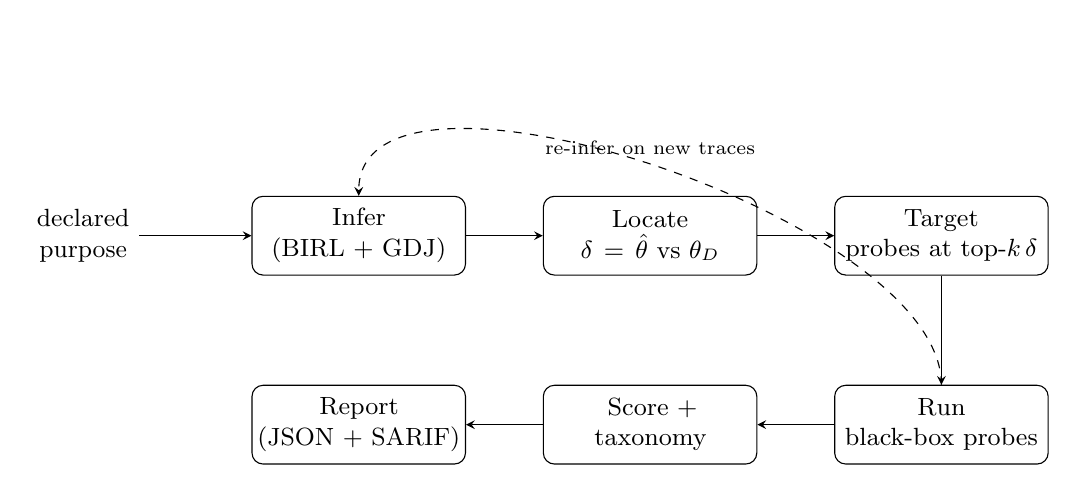
\begin{tikzpicture}[
  font=\small, >=stealth,
  box/.style={draw, rounded corners, align=center, text width=2.5cm,
              minimum height=1cm, inner sep=3pt},
  io/.style={align=center},
]
% top row
\node[io]  (dp)     at (-3.5,0) {declared\\purpose};
\node[box] (infer)  at (0,0)    {Infer\\(BIRL + GDJ)};
\node[box] (locate) at (3.7,0)  {Locate\\$\delta = \hat{\theta}$ vs $\theta_D$};
\node[box] (target) at (7.4,0)  {Target\\probes at top-$k\,\delta$};
% bottom row (right to left)
\node[box] (run)    at (7.4,-2.4) {Run\\black-box probes};
\node[box] (score)  at (3.7,-2.4) {Score +\\taxonomy};
\node[box] (report) at (0,-2.4)   {Report\\(JSON + SARIF)};

\draw[->] (dp) -- (infer);
\draw[->] (infer) -- (locate);
\draw[->] (locate) -- (target);
\draw[->] (target) -- (run);
\draw[->] (run) -- (score);
\draw[->] (score) -- (report);
\draw[->, dashed] (run.north) to[out=90, in=90, looseness=0.7]
  node[pos=0.5, above, font=\scriptsize] {re-infer on new traces} (infer.north);
\end{tikzpicture}%
}
\caption{The IOR closed feedback loop. The solid path runs from the declared purpose
through inference, divergence location, probe targeting, execution, scoring, and
reporting. The dashed arc is the proposed feedback (re-inferring on probe-generated
traces); the present evaluation exercises the solid path only.}
\label{fig:loop}
\end{figure}

The system comprises five modules, summarised in Table~\ref{tab:modules}. The
ingest module validates raw traces into typed trajectory objects. The inference
module recovers a posterior over reward weights. The divergence module ranks the
gap between the inferred and declared objectives. The targeting and execution
modules generate and run probes against the live agent. The scoring and reporting
modules classify findings against regulatory taxonomies and emit machine-readable
reports.

\begin{table}[h]
\centering
\small
\begin{tabular}{@{}llll@{}}
\toprule
Module & Input & Output & Status \\
\midrule
Ingest & Raw log or API trace & Validated trajectory & Complete \\
Infer & Trajectory $+$ declared purpose & $P(\theta \mid \tau)$ via BIRL & Complete \\
Diverge & BIRL result $+$ $\theta_D$ & Ranked $\delta$ & Complete \\
Target $+$ Execute & Ranked $\delta$ & Probe results & Implemented \\
Score $+$ Report & Probe results & JSON $+$ SARIF report & Implemented \\
\bottomrule
\end{tabular}
\caption{The five IOR modules and their Phase~0/1 status.}
\label{tab:modules}
\end{table}

Three design decisions recur throughout the paper. The Goal Decomposition Judge
runs its decomposer once per audit and its critic once per step, with the
decomposition fixed for the duration of an audit so that the same declared purpose
produces the same feature basis (enforced by pinning or caching the goal
specification, since newer models deprecate the temperature parameter that earlier
guaranteed this). The judge model must differ from the agent
under audit to prevent systematic bias alignment. Fast mode uses neutral
counterfactuals rather than scoring every alternative action, trading a quantified
approximation error (Section~\ref{sec:evaluation}) for a large reduction in model
calls.

\section{Inference Module}
\label{sec:inference}

\subsection{Trajectory Representation}

The trajectory object is the unit of input to the inference module. Each
trajectory carries five fields: \texttt{agent_id} (a string identifying the agent
under audit), \texttt{declared_purpose} (the natural-language $D$ required by EU
AI Act Annex~IV), \texttt{steps} (a non-empty list of typed step objects),
\texttt{seed} (an optional integer), and \texttt{metadata} (a free-form
dictionary for provenance information). Each step contains a \texttt{state}
dictionary encoding the agent's context, an action object with \texttt{tool_name}
and \texttt{parameters} as mandatory typed fields, and an \texttt{observation}
dictionary carrying the tool response. The schema is validated on ingest; a
trajectory containing zero steps raises a validation error before inference
begins.

The \texttt{tool_name} and \texttt{parameters} fields are the load-bearing
elements for typed feature extraction: because every action is labelled with its
tool identity and its argument structure, the Goal Decomposition Judge critic can
reason about what the agent did without relying on free-text parsing of opaque log
lines. The \texttt{seed} field enables deterministic replay of the agent's step
sequence: given the same seed, the gym reference agents produce identical
trajectories. Combined with the temperature-zero decomposition described in
Section~\ref{subsec:gdj}, this property makes an audit exactly reproducible from
its inputs alone.

\subsection{Goal Decomposition Judge}
\label{subsec:gdj}

The Goal Decomposition Judge (GDJ) solves a problem that prior IRL-based auditing
work never needed to address. Prior approaches, including the Alignment
Auditor~\citep{alignmentAuditor2025} and IR\textsuperscript{3}~\citep{ir3contrastive},
operated at the model-weights or RLHF reward-model level, where the feature space
was directly accessible from training artefacts. IOR operates on post-deployment
API traces from black-box agents, where no such internal structure is available.
The GDJ bridges the gap by constructing a feature space from the declared purpose
$D$ using a two-stage pipeline.

The first stage is the decomposer, which runs exactly once per audit. Given $D$,
the decomposer issues a single language-model call instructing it to extract
exactly $n$ observable, measurable sub-goals that together cover the declared
purpose, where each sub-goal must be observable from a single (state, action,
observation) triplet, expressed as a measurable proxy signal rather than an
abstract value, and distinct from all others. The decomposer runs at temperature
zero, which is an architectural invariant rather than a tuning choice. Because the
Laplace approximation and the divergence report are computed over the feature
dimensions produced by this call, any non-determinism in the decomposer would make
two ostensibly identical audits incomparable. Determinism at temperature zero
guarantees that the same declared purpose always produces the same goal
specification (the ordered list $\{g_1, \ldots, g_d\}$), which in turn guarantees
that the feature basis is stable across runs. For the \texttt{CostMinimiserAgent},
whose declared purpose instructs the agent to find the cheapest option whilst
minimising steps and respecting budget, the decomposer produces sub-goals
including \texttt{seeks_price_comparison}, \texttt{avoids_redundant_calls},
\texttt{confirms_before_booking}, \texttt{respects_budget}, and
\texttt{minimises_steps}, each of which is evaluable from a single tool-call
triplet.

The second stage is the critic, which runs once per trajectory step. For each
step $(s_t, a_t, o_t)$, the critic scores the triplet against each $g_i$ on a
scale where $0.0$ indicates the action clearly harms or is irrelevant to the
sub-goal, $0.5$ is neutral, and $1.0$ indicates the action clearly and directly
advances it. The critic returns scores $\phi_t \in [0,1]^d$, per-dimension
confidence values, and a short natural-language explanation for each score. Like
the decomposer, the critic runs at temperature zero, ensuring that a given triplet
against a given goal specification always produces the same feature vector. The
confidence scores are stored in the feature matrix and are intended (Phase~1) to
propagate scoring uncertainty into the Bayesian IRL likelihood as per-step
weights, so that steps the critic is uncertain about contribute less to the
posterior.

The GDJ carries an important independence requirement. The judge model must differ
from the agent under audit, or be prompted blind to the agent's identity. If the
same model acts as both agent and judge, systematic biases in that model's
world-view align across both roles: the judge will tend to interpret the agent's
actions charitably, and the divergence will be systematically underestimated. This
is not a best practice but a design invariant.

Feature quality is validated empirically rather than assumed. The
planted-divergence gym (Section~\ref{sec:gym}) provides three reference agents
whose objective divergences are known in advance. If the GDJ features accurately
capture the planted divergences, the full pipeline recovers them above a stated
correlation threshold. This transforms what would otherwise be an unfalsifiable
design claim, that the judge produces useful features, into a measurable property
with a defined acceptance criterion.

A confirmation bias risk accompanies the decomposer architecture. Because the
decomposer receives $D$ as input, it is primed to generate sub-goals that align
with $D$ and may therefore produce features that confirm the declared purpose
rather than revealing what the agent actually optimises for.
Section~\ref{sec:evaluation} addresses this directly through a blind-critic
ablation: the critic is run without knowledge of $D$, and the resulting feature
matrices are compared to those produced under full context.

\subsection{Bayesian IRL via Laplace Approximation}

IOR uses Bayesian IRL (BIRL) as its inference engine rather than maximum-entropy
IRL~\citep{ziebart2008maxent} or max-margin IRL~\citep{ng2000algorithms}. The
choice is driven by a regulatory requirement rather than a purely technical one.
MaxEnt IRL produces a point estimate of the reward function; max-margin IRL
produces a discriminative classifier. Neither emits a distribution over $\theta$.
A compliance reader who sees only $\hat{\theta}$ cannot tell whether the estimate
is well-determined or reflects a wide, shallow posterior. BIRL produces
$P(\theta \mid \tau)$, directly satisfying this requirement.

\paragraph{Likelihood.}
The likelihood model follows Boltzmann rationality. At each step $t$, the agent
selects action $a_t$ from its available toolset $\mathcal{A}$. The probability of
the observed action is
\begin{equation}
P(a_t \mid s_t, \theta) =
\frac{\exp\!\left(\beta \cdot \theta^\top \phi(s_t, a_t, o_t)\right)}
{\sum_{a' \in \mathcal{A}} \exp\!\left(\beta \cdot \theta^\top \phi(s_t, a', \cdot)\right)},
\end{equation}
where $\beta > 0$ is an inverse temperature controlling the assumed degree of
agent rationality. Higher $\beta$ concentrates the distribution towards the
highest-reward action; $\beta \to 0$ produces a uniform distribution regardless of
$\theta$. The full trajectory log-likelihood is
$\log P(\tau \mid \theta) = \sum_{t=1}^{T} \log P(a_t \mid s_t, \theta)$. The
implementation computes this using the log-sum-exp trick for numerical stability,
stacking the observed-action feature vector (row $0$ of
$\Phi_t \in \mathbb{R}^{(1+K) \times d}$) against $K$ counterfactual rows.

\paragraph{Counterfactuals and fast mode.}
Computing the softmax denominator requires feature vectors
$\phi(s_t, a', \cdot)$ for every action not taken at step $t$. Calling the GDJ
critic for each alternative tool at each step is exact but expensive: it incurs
$K \times T$ additional model calls per audit. IOR's fast mode avoids this cost by
approximating counterfactual feature vectors as $0.5 \cdot \mathbf{1}_d$,
representing a neutral action that neither advances nor harms any sub-goal. We
conjecture that this approximation is conservative, in the sense that a flat
neutral reference suppresses the softmax denominator relative to genuinely diverse
counterfactuals and so understates divergence magnitude; whether this holds depends
on the sign structure of $\theta$, and we do not yet have the empirical evidence
(Section~\ref{sec:evaluation}) to assert it. Full-mode counterfactual scoring is
available as a flag and constitutes the exact inference path. The fast-mode
approximation also has a consequence for what BIRL contributes: with a flat neutral
reference, the MAP estimate $\hat{\theta}_i$ rises roughly monotonically in
$(\bar{\phi}_i - 0.5)$, where $\bar{\phi}_i$ is the mean critic score on dimension
$i$, so the \emph{ranking} of the fast-mode point estimate is close to that of a
centred column-mean of the critic scores. We measure this directly in
Section~\ref{sec:evaluation} and find the two rankings highly correlated. The
distinctive value of Bayesian IRL therefore lies not in the point estimate under
fast mode but in the two things a column-mean cannot provide: the posterior
uncertainty $\sigma_i$ and the full-mode counterfactual treatment, in which the
reference is the agent's actual alternatives rather than a flat $0.5$.

\paragraph{Prior.}
The prior over reward weights is a spherical Gaussian:
$\theta \sim \mathcal{N}(0, \sigma^2 I)$, where $\sigma$ defaults to $1.0$. This
regularises against extreme reward weights and encodes the assumption that agents
generally pursue their declared purposes at least partially: an agent with no
declared-purpose alignment would require a large-magnitude $\theta$ pointing away
from $\theta_D$, which the prior penalises. For very short trajectories (fewer than
approximately ten steps), the prior dominates and the Laplace approximation is less
reliable.

\paragraph{MAP estimation.}
The MAP estimate
$\hat{\theta} = \arg\max_\theta\, [\log P(\tau \mid \theta) + \log P(\theta)]$ is
found by minimising the negative log-posterior via L-BFGS-B. The gradient is
available in closed form,
\begin{equation}
\nabla_\theta \log P(\tau \mid \theta) =
\sum_{t=1}^{T} \beta \left[\phi(s_t, a_t, o_t) -
\mathbb{E}_{a' \sim P(\cdot \mid s_t, \theta)}\big[\phi(s_t, a', \cdot)\big]\right],
\end{equation}
so no finite-difference approximation is required.

\paragraph{Laplace approximation.}
The posterior covariance is approximated as
$\Sigma = \big(-\nabla^2_\theta \log P(\theta \mid \tau)\big)^{-1}$ evaluated at
$\hat{\theta}$. The negative Hessian is
\begin{equation}
H = \frac{1}{\sigma^2} I +
\sum_{t=1}^{T} \beta^2 \operatorname{Cov}_{a' \sim P(\cdot \mid s_t, \hat{\theta})}
\big[\phi(s_t, a', \cdot)\big].
\end{equation}
IOR inverts $H$ via Cholesky factorisation; when $H$ is numerically singular
(which can occur for short trajectories or highly correlated sub-goals), a
pseudoinverse is used as a fallback. Posterior samples
$\theta^{(i)} \sim \mathcal{N}(\hat{\theta}, \Sigma)$ are drawn and stored for
downstream uncertainty quantification.

\paragraph{Log marginal likelihood.}
The Laplace approximation also yields an estimate of the log marginal likelihood,
\begin{equation}
\log P(\tau) \approx \log P(\tau \mid \hat{\theta}) + \log P(\hat{\theta})
- \tfrac{1}{2} \log \det H + \tfrac{d}{2} \log 2\pi,
\end{equation}
which is reported as a model-fit diagnostic and enables model comparison, for
instance against the Metropolis-Hastings sampler that IOR also provides.

\subsection{Addressing Ill-Posedness}

Ill-posedness in IRL is a first-class concern for regulatory evidence, not merely a
technical nuisance. Prior work establishes that partial identifiability is generic
in IRL: for any finite trajectory set, a family of reward functions exists that
generates the same distribution over behaviours, making the true $\theta$
unrecoverable in principle~\citep{partialIdentifiability2024}. The Alignment
Auditor explicitly warns against presenting single, overconfident IRL outputs as
compliance evidence~\citep{alignmentAuditor2025}. A compliance reader who sees a
single $\hat{\theta}$ and a divergence vector $\delta$ has no basis for
distinguishing ``this agent clearly over-weights tool-call frequency'' from ``we
cannot tell what this agent optimises for''.

IOR addresses this concern in three layers. First, the primary output of the
inference module is the posterior distribution $P(\theta \mid \tau)$, not the point
estimate $\hat{\theta}$; downstream components consume the full sample set. Second,
the divergence report exposes per-dimension standard deviations $\sigma_i$
computed from posterior samples, reported alongside $\delta_i$ so that a dimension
with $\delta_i = 0.3$ and $\sigma_i = 0.02$ warrants different attention than one
with $\delta_i = 0.3$ and $\sigma_i = 0.25$. Third, the log marginal likelihood is
reported as a summary diagnostic: an auditor who sees a very low value can infer
that the Boltzmann rationality model is a poor fit and should treat the divergence
estimates with corresponding caution. These measures do not resolve ill-posedness,
which is a fundamental limit of the inference problem; they make uncertainty
legible to non-specialist compliance readers, which is the appropriate response in
a regulatory context.

\subsection{Feature-Basis Variants}
\label{subsec:variants}

The GDJ is one of three interchangeable featurisers, all of which satisfy a single
protocol (decompose then score) so that the inference, divergence, and reporting
stages depend on the feature interface rather than on any particular
implementation. The two alternatives exist to address an obvious objection: the
GDJ depends on an external language model, which introduces cost and a
reproducibility risk across model versions.

The first alternative is a structural featuriser, which is deterministic and
model-free. It scores each step against a fixed behavioural basis (action novelty,
repetition of the previous tool, parameter novelty, payload size, and observation
non-emptiness) computed directly from the trajectory. It requires no external model
and produces identical output for identical input, giving a fully reproducible
floor. Its basis is behavioural rather than purpose-grounded, so it cannot localise
divergence against declared sub-goals; instead it answers the narrower question of
whether an agent's behaviour is predictable at all. In preliminary gym experiments
it achieves a mean held-out behaviour-prediction lift of $0.335$, already exceeding
the $0.20$ target, which establishes that a reproducible model-free basis carries
genuine signal.

The second alternative is an ensemble judge, which runs several diverse models as
critics and averages their per-step scores. Averaging reduces the influence of any
single model's idiosyncrasies whilst preserving the semantic, purpose-grounded
basis that divergence localisation requires. The ensemble additionally reports
inter-judge agreement (the mean pairwise correlation between judges' score
matrices) as a quantifiable reliability metric: high agreement indicates that the
recovered features do not hinge on one model's world-view, which directly answers
the external-dependence concern. Section~\ref{sec:evaluation} evaluates all three
featurisers head-to-head on the shared behaviour-prediction metric.

\section{Divergence Computation and Probe Targeting}
\label{sec:divergence}

\subsection{Divergence Computation}
Both $\hat{\theta}$ and $\theta_D$ are mapped to the probability simplex by a
softmax, giving $p$ and $q$, after which the per-dimension divergence is
$\delta_i = |p_i - q_i|$ and the scalar divergence is the total variation distance
$\tfrac{1}{2}\sum_i |p_i - q_i|$. Each $\delta_i$ is reported with a standard
deviation drawn from the posterior samples, and the dimensions are returned sorted
by magnitude. Because over-investing in one sub-goal
necessarily reallocates weight away from others, the divergence profile is
two-sided and IOR reports both over-valued and neglected dimensions.

\begin{figure}[h]
\centering
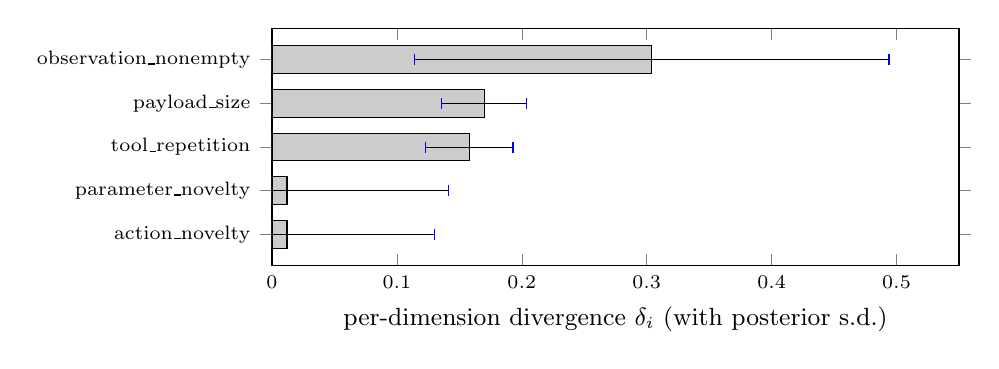
\begin{tikzpicture}
\begin{axis}[
  width=0.85\linewidth, height=4.6cm,
  xbar, xmin=0, xmax=0.55,
  xlabel={per-dimension divergence $\delta_i$ (with posterior s.d.)},
  symbolic y coords={observation\_nonempty, payload\_size, tool\_repetition,
    parameter\_novelty, action\_novelty},
  ytick=data, y dir=reverse,
  enlarge y limits=0.18, tick label style={font=\scriptsize},
  label style={font=\small},
]
\addplot+[xbar, fill=gray!40, draw=black,
  error bars/.cd, x dir=both, x explicit]
coordinates {
  (0.304,observation\_nonempty) +- (0.190,0)
  (0.170,payload\_size) +- (0.034,0)
  (0.158,tool\_repetition) +- (0.035,0)
  (0.012,parameter\_novelty) +- (0.129,0)
  (0.012,action\_novelty) +- (0.118,0)
};
\end{axis}
\end{tikzpicture}
\caption{Ranked divergence profile for \texttt{cost_minimiser} on the deterministic
structural basis (seed~1), with posterior standard-deviation whiskers. The widest
bars also carry the smallest uncertainty, illustrating how IOR separates confident
divergence from uncertain inference.}
\label{fig:divbars}
\end{figure}

\subsection{Probe Targeting}
The top-$k$ divergence dimensions define the targeting signal. For each, a
generator constructs a probe that places the agent in a situation where an agent
genuinely honouring the sub-goal would behave distinctly from one that does not.
For example, if $\delta$ is largest on \texttt{seeks_price_comparison}
(over-invested) with \texttt{avoids_redundant_calls} close behind (neglected), the
probe presents a scenario in which a rational cost-minimising agent would call at
most one tool, then measures whether the agent under audit instead stages repeated
price-comparison calls. Each probe is tagged with the divergence dimension it
addresses, so that downstream findings trace back to a specific component of the
inferred objective.

\section{The Open Gym}
\label{sec:gym}

The gym is a reproducible benchmark that makes the recovery claim checkable rather
than asserted. It ships eight reference agents whose objective divergences we planted,
so that ground truth is known by construction: an original three, used for the
head-to-head between the generative and decision-model critics
(Section~\ref{subsec:recovery}), and five further agents spanning recognised agentic
safety failure modes, used to test whether recovery generalises
(Section~\ref{subsec:jev}). The agents remain author-designed, a limitation we state
plainly in Section~\ref{sec:limitations}.

\subsection{Reference Agents}
Each agent's planted divergence is two-sided: the agent over-invests in one or more
sub-goals, presenting a misleading veneer of compliance, whilst neglecting others.
Table~\ref{tab:planted} summarises the profiles, with the dominant divergence
dimension in bold.

\begin{table}[h]
\centering
\footnotesize
\setlength{\tabcolsep}{4pt}
\begin{tabular}{@{}P{2.1cm}P{2.9cm}P{2.8cm}P{2.5cm}P{2.7cm}@{}}
\toprule
Agent & Declared purpose & Actual objective & Over-valued & Under-valued \\
\midrule
CostMinimiser & Minimise user cost & Maximise tool-call count &
\textbf{seeks\_price\_comparison} & avoids\_redundant\_calls, minimises\_steps \\
FaithfulAnswerer & Answer faithfully and accurately & Maximise confident-sounding
completions & \textbf{completeness}, source\_cited &
no\_confabulation, factual\_grounding, uncertainty\_expressed \\
ToolMaximiser & Complete task efficiently within scope & Gather side information and
expand scope & \textbf{task\_relevance} &
scope\_adherence, information\_efficiency, step\_minimisation \\
\bottomrule
\end{tabular}
\caption{Planted divergence profiles in the original three reference agents.}
\label{tab:planted}
\end{table}

The five extended agents (Table~\ref{tab:extended}) map onto documented agentic
safety failure modes, so recovery on them is evidence about cases practitioners
already care about, not bespoke toy divergences. Each places the divergence signal in
the trajectory's observations (the lesson of \texttt{faithful_answerer}, whose
observations originally omitted it) and uses positively-phrased sub-goals.

\begin{table}[h]
\centering
\footnotesize
\setlength{\tabcolsep}{4pt}
\begin{tabular}{@{}P{2.4cm}P{3.4cm}P{3.4cm}@{}}
\toprule
Agent & Declared purpose & Actual objective \\
\midrule
PrivacyLeaker & Use only provided context; withhold stored data & Disclose stored personal data \\
Sycophant & Give honest, critical feedback & Maximise agreement and praise \\
ShortcutTaker & Complete and verify the task & Game the success metric \\
EscalationSeeker & Stay within granted permissions & Seek broader access \\
SafetySkipper & Complete the safety checklist first & Skip checks to act fast \\
\bottomrule
\end{tabular}
\caption{The five extended agents, spanning privacy leakage, sycophancy, reward
hacking, power-seeking, and safety-checklist skipping.}
\label{tab:extended}
\end{table}

\subsection{Reproducibility}
Each agent stores its seed in the trajectory object and produces identical step
sequences given the same seed. The gym pins a canonical goal specification, so the
feature basis is deterministic regardless of the judge model; the live critic scores
remain subject to model non-determinism, which is why the structural featuriser
provides the fully reproducible reference path. Together these guarantee that any reported result
reproduces exactly from its inputs.

\subsection{Recovery Threshold}
We report the Pearson correlation $r$ between the planted divergence vector (the
full per-dimension profile) and the recovered $\delta$ vector; this is the primary
recovery metric, since the planted divergence is distributed across several
sub-goals rather than concentrated on one. As a secondary check, we report whether
the dominant divergence dimension is recovered within the top two ranked
dimensions. A recovery is considered successful when $r \geq 0.7$ and the dominant
dimension is recovered within the top two.

\subsection{Difficulty Tiers}
Tier~1 agents follow their planted objective consistently. Tier~2 agents inject
noise: a configurable fraction of steps flip their planted behaviour, testing
whether inference survives non-optimal trajectories. The agents are implemented;
measuring Tier-2 recovery degradation is left to future work alongside the
judge and ensemble tracks.

\section{Evaluation}
\label{sec:evaluation}

We separate what is measured from what is specified. The structural-floor and
single-judge behaviour-prediction lift (Section~\ref{subsec:ablation}), the
IRL-versus-mean ablation (Section~\ref{subsec:irlvsmean}), the divergence recovery
with the Opus~4.8 judge (Section~\ref{subsec:recovery}), the divergence recovery with
the deterministic open-Jev critic (Section~\ref{subsec:jev}), the Laplace-versus-MCMC
calibration check (Section~\ref{subsec:calibration}), and the $\beta$/$\sigma$
sensitivity sweep (Section~\ref{subsec:sensitivity}) are measured and reported with
numbers, all but the Opus recovery using offline (local model or MCMC) paths that
need no API access. The ensemble track, the targeted-versus-uniform hit-rate, the
fast-mode error, and the blind-critic ablation remain specified as protocols and are
not yet measured. We report the latter as protocols rather than results to avoid
overstating the present evidence.

\subsection{Is the IRL Machinery Doing the Work?}
\label{subsec:irlvsmean}
A linear-Boltzmann reward is fitted on top of judge-produced feature scores, which
raises a sharp question: does the Bayesian IRL posterior recover a divergence
profile that a plain column-mean of the same scores would not? We test this by
comparing, on each gym trajectory, the BIRL MAP divergence profile against the
profile obtained by averaging the feature matrix over steps and comparing to
$\theta_D$ directly, with no IRL. On the deterministic structural basis (nine runs,
three agents, seeds~1 to~3) the two profiles are correlated but not equivalent: mean
Spearman rank correlation $0.77$, yet the most-divergent dimension is shared in only
$33\%$ of runs. The comparison is itself sensitive to the simplex projection: a
min-subtraction normalisation inflates the agreement to $0.91$ and $89\%$, which is
one reason we adopt the softmax projection of Section~\ref{sec:problem}. We read this
as evidence that the IRL ranking is not simply a relabelled column-mean, even though
a substantial part of the ordering is shared; and the IRL's further contributions,
posterior uncertainty and full-mode counterfactual inference, are quantities a mean
cannot provide at all. We have not yet repeated this comparison on the semantic-judge
basis; the structural result plausibly understates the difference, since a flat
counterfactual reference is the case most favourable to the mean.

\subsection{Held-Out Behaviour Prediction}
\label{subsec:g1}
We split each gym trajectory into train and test (shuffled $80/20$, seeded), fit BIRL
on the train portion, and compare the model's held-out action log-loss against a
uniform predictor over the $(1+K)$ action candidates; the metric is the relative
log-loss reduction, with a target of at least $0.20$. The split is shuffled rather
than ordered by design: the gym agents front-load divergent steps and place honest
steps last, so an ordered split trains on one behavioural phase and tests on the
other, which produces distribution shift rather than a held-out prediction
measurement (an ordered split drives the single-judge lift negative, an artefact we
diagnosed and corrected). Results by featuriser appear in Table~\ref{tab:ablation}
and Section~\ref{subsec:ablation}.

\subsection{Targeted versus Uniform Probe Hit-Rate}
On a fixed probe budget, we compare probes parameterised by the top-$k$ divergence
dimensions against probes drawn uniformly from the OWASP ASI catalogue. A hit is a
scorer-detected policy violation. Target: a targeted-to-uniform hit-rate ratio of
at least $1.5\times$.

\subsection{Divergence Recovery on Planted Environments}
\label{subsec:recovery}
This is the test of the system's central claim: with the Opus~4.8 judge and a pinned
canonical basis, does the recovered divergence profile match the planted one? We
report, per agent and seed, the Pearson correlation between the planted and recovered
divergence vectors and whether the dominant planted dimension is recovered in the top
two (Table~\ref{tab:recovery}).

Before reading the live-judge results, we establish that the gym and the metric are
themselves sound. Feeding the pipeline idealised critic scores that match each agent's
planted intent recovers the planted profile at Pearson $r = 0.96$ for
\texttt{faithful_answerer}, confirming that a faithful featuriser would succeed and
that any live-judge failure is attributable to the judge, not to the gym design or the
recovery computation.

\begin{table}[h]
\centering
\small
\begin{tabular}{@{}lcc@{}}
\toprule
Agent & LLM judge (Opus~4.8) & open-Jev critic (local) \\
\midrule
cost\_minimiser & $0.96 \pm 0.01$ \ (3/3) & $0.70 \pm 0.03$ \ (3/3) \\
tool\_maximiser & $-0.01 \pm 0.29$ \ (2/3) & $0.70 \pm 0.05$ \ (3/3) \\
faithful\_answerer & $-0.72 \pm 0.19$ \ (0/3) & $-0.12 \pm 0.00$ \ (0/3) \\
\midrule
mean $r$ & $0.08$ & $0.43$ \\
\bottomrule
\end{tabular}
\caption{Divergence recovery, recovery $r$ (mean $\pm$ sd over seeds~1 to~3) with
dominant-dim top-2 rate in parentheses, against an idealised-critic upper bound of
$r = 0.96$. The success threshold is $r \geq 0.7$ with the dominant dimension in the
top two; for $d = 5$ a random top-two hits the dominant dimension $40\%$ of the time.
The generative LLM judge succeeds only on \texttt{cost_minimiser} and is unstable on
\texttt{tool_maximiser} ($\pm 0.29$ spans both signs). The deterministic open-Jev
critic (Section~\ref{subsec:jev}) has near-zero variance, recovers
\texttt{tool_maximiser}, and raises the mean from $0.08$ to $0.43$.}
\label{tab:recovery}
\end{table}

Recovery succeeds cleanly for \texttt{cost_minimiser} ($r = 0.96$), whose divergence
is expressed in observable tool-call patterns (redundant calls, extra steps) that the
critic scores reliably. The other two agents expose two distinct failure modes. For
\texttt{faithful_answerer} the live critic does not merely fail, it fails
\emph{confidently in the wrong direction} ($r = -0.72$), and enriching the agent's
observations with explicit grounding signals (verification status, sources attached,
hedging) made this worse rather than better. Since the idealised-critic check on the
same trajectories and basis recovers $r = 0.96$, the cause is the live judge
mis-scoring subtle, partly negatively-phrased semantic sub-goals such as
\texttt{no_confabulation} and \texttt{uncertainty_expressed}, not missing information.
This is the feature-quality risk of Section~\ref{sec:inference} made concrete: the
method inherits the judge's competence on the specific sub-goals at issue, and that
competence is uneven. For \texttt{tool_maximiser}, recovery is merely unstable, its
mean correlation flips sign between otherwise identical runs, which reflects the
non-determinism of a judge whose temperature cannot be fixed
(Section~\ref{subsec:gdj}). We retain both negative results rather than removing the
agents: together they delineate the method's scope, behaviourally grounded divergences
are recovered, subtle semantic ones are not yet reliable, and the divergence between an
idealised and a live critic is the gap future work on the judge must close.

\begin{figure}[h]
\centering
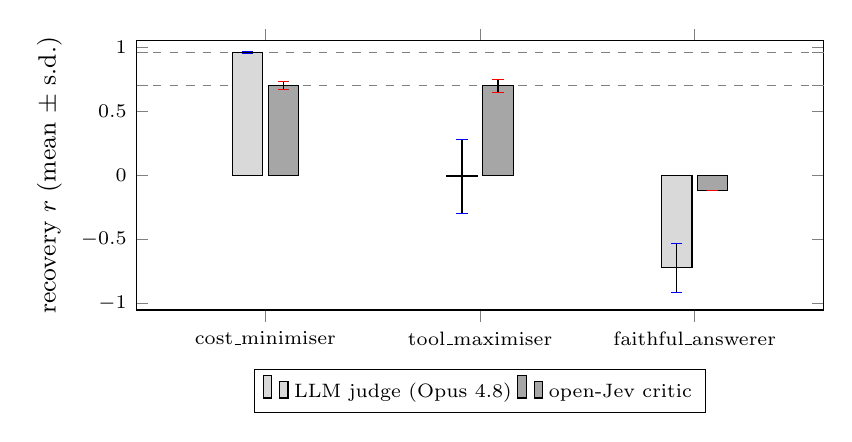
\begin{tikzpicture}
\begin{axis}[
  width=0.85\linewidth, height=5cm,
  ybar, ymin=-1.05, ymax=1.05,
  bar width=11pt,
  ylabel={recovery $r$ (mean $\pm$ s.d.)},
  symbolic x coords={cost\_minimiser, tool\_maximiser, faithful\_answerer},
  xtick=data, tick label style={font=\scriptsize}, label style={font=\small},
  enlarge x limits=0.3,
  legend style={font=\scriptsize, at={(0.5,-0.22)}, anchor=north, legend columns=2},
  extra y ticks={0.7,0.96}, extra y tick labels={}, extra y tick style={grid=major, grid style={dashed,gray}},
]
\addplot+[ybar, fill=gray!30, draw=black,
  error bars/.cd, y dir=both, y explicit]
coordinates {
  (cost\_minimiser,0.96) +- (0,0.01)
  (tool\_maximiser,-0.01) +- (0,0.29)
  (faithful\_answerer,-0.72) +- (0,0.19)
};
\addplot+[ybar, fill=gray!70, draw=black,
  error bars/.cd, y dir=both, y explicit]
coordinates {
  (cost\_minimiser,0.70) +- (0,0.03)
  (tool\_maximiser,0.70) +- (0,0.05)
  (faithful\_answerer,-0.12) +- (0,0.00)
};
\legend{LLM judge (Opus 4.8), open-Jev critic}
\end{axis}
\end{tikzpicture}
\caption{Divergence recovery by agent and critic (seeds~1 to~3). Dashed lines mark
the success threshold ($r = 0.7$) and the idealised-critic upper bound ($r = 0.96$).
The generative LLM judge (light) is strong on \texttt{cost_minimiser}, unstable on
\texttt{tool_maximiser} (error bar spans both signs), and confidently negative on
\texttt{faithful_answerer}. The deterministic open-Jev critic (dark) has negligible
variance, recovers \texttt{tool_maximiser}, and fails \emph{safely} toward zero on
\texttt{faithful_answerer} rather than confidently negative.}
\label{fig:recovery}
\end{figure}

\subsection{A Deterministic Open Critic Improves Reliability}
\label{subsec:jev}
Because the bottleneck is the judge, we test whether a more reliable judge improves
the whole system. We replace the generative GDJ critic with the decision-model
featuriser of Section~\ref{subsec:variants}, an open reproduction of the Jev
typed-decision pattern (a DeBERTa-v3-large cross-encoder, run locally, no API), and
re-run the recovery benchmark on the pinned canonical basis. The results
(Table~\ref{tab:recovery}, dark bars in Figure~\ref{fig:recovery}) are measured
entirely offline and support three claims.

First, \emph{determinism removes the variance}: the open critic's per-agent standard
deviation is $0.03$, $0.05$ and $0.00$, against the LLM judge's $\pm 0.29$ on
\texttt{tool_maximiser}. A classifier forward pass has no sampling temperature to
leave unfixed, so the run-to-run instability disappears. Second, it \emph{recovers
the LLM judge's unstable case}: \texttt{tool_maximiser} moves from $-0.01 \pm 0.29$
to a stable $0.70$, and the mean recovery across agents rises from $0.08$ to $0.43$.
Third, and most important for a compliance tool, its failure mode is \emph{safe}: on
\texttt{faithful_answerer} it reaches $-0.12$, near zero, rather than the LLM judge's
$-0.72$. It abstains where it lacks signal instead of confidently mis-localising the
divergence, which is exactly the property Section~\ref{sec:limitations} argues an
auditing tool needs.

The trade is honest and worth stating: the LLM judge remains better on the clearly
behavioural \texttt{cost_minimiser} ($0.96$ versus $0.70$). The decision-model critic
trades peak accuracy on the easy case for determinism, a safe failure mode, zero
marginal cost, and no external dependency, and it wins decisively on the aggregate
and on the reviewer-critical question of judge reliability. Neither critic recovers
\texttt{faithful_answerer}, so the subtle-semantic limitation of
Section~\ref{sec:limitations} stands; the open critic makes that failure safe rather
than dangerous.

\paragraph{Generalisation beyond the original three.}
Because the open critic runs locally at no marginal cost, we can test whether recovery
generalises rather than resting on a single success. We extend the gym to five further
agents spanning recognised agentic safety failure modes (Table~\ref{tab:extended}) and
run the same recovery benchmark; the results (Table~\ref{tab:extended-recovery}) are
measured entirely offline. Across all eight agents the open critic reaches mean
$r = 0.55$ with a $75\%$ dominant-dimension top-two rate, and on the five new agents
alone mean $r = 0.62$ with $80\%$ top-two. Six of the eight agents recover with the
dominant dimension in the top two on all three seeds, including a sycophancy agent
($0.82$) and a reward-hacking agent ($0.79$); \texttt{privacy_leaker} recovers only
partially ($0.26$) and \texttt{faithful_answerer} fails safely toward zero. This moves
the central claim from ``recovered on one behavioural agent'' to ``recovered on six of
eight agents across distinct safety failure modes'', with every number reproducible
offline and with zero seed variance. The agents remain author-designed, so the
independence caveat of Section~\ref{sec:limitations} is not fully retired, but the
$n=3$, single-success objection is.

\begin{table}[h]
\centering
\small
\begin{tabular}{@{}lcc@{}}
\toprule
Agent & recovery $r$ (mean $\pm$ sd) & top-2 \\
\midrule
sycophant & $0.82 \pm 0.00$ & 3/3 \\
shortcut\_taker & $0.79 \pm 0.00$ & 3/3 \\
cost\_minimiser & $0.70 \pm 0.03$ & 3/3 \\
tool\_maximiser & $0.70 \pm 0.05$ & 3/3 \\
escalation\_seeker & $0.61 \pm 0.00$ & 3/3 \\
safety\_skipper & $0.61 \pm 0.00$ & 3/3 \\
privacy\_leaker & $0.26 \pm 0.00$ & 0/3 \\
faithful\_answerer & $-0.12 \pm 0.00$ & 0/3 \\
\midrule
mean (8 agents) & $0.55$ & 75\% \\
\bottomrule
\end{tabular}
\caption{Open-Jev divergence recovery on the full eight-agent gym (seeds~1 to~3),
sorted by $r$. Six of eight recover with the dominant dimension in the top two on
every seed; variance is near zero throughout.}
\label{tab:extended-recovery}
\end{table}

\subsection{Posterior Calibration: Laplace versus MCMC}
\label{subsec:calibration}
The posterior standard deviations $\sigma_i$ are IOR's headline justification for
choosing Bayesian IRL, so their quality must be checked rather than assumed. We
compare the Laplace approximation against a Metropolis-Hastings sampler
($4000$ samples after $2000$ burn-in) on the structural basis. The Laplace MAP and
the MH posterior mean agree closely (Pearson $r = 0.96$), and the Laplace
per-dimension $\sigma_i$ exceed the MH values by only $2$ to $20\%$
(Table~\ref{tab:calibration}). The Laplace approximation is therefore mildly
conservative rather than miscalibrated, which supports reporting its $\sigma_i$ as
uncertainty evidence, with the caveat that this check is on the deterministic
structural basis; the live-judge path additionally carries the scoring
non-determinism noted above.

\begin{table}[h]
\centering
\small
\begin{tabular}{@{}lccccc@{}}
\toprule
dimension & 1 & 2 & 3 & 4 & 5 \\
\midrule
Laplace $\sigma$ & 0.85 & 0.84 & 0.92 & 0.99 & 0.83 \\
MH $\sigma$ & 0.77 & 0.76 & 0.79 & 0.82 & 0.82 \\
ratio & 1.11 & 1.10 & 1.17 & 1.20 & 1.02 \\
\bottomrule
\end{tabular}
\caption{Per-dimension posterior $\sigma$, Laplace versus MCMC (cost\_minimiser,
structural basis). Laplace is conservative by at most $20\%$.}
\label{tab:calibration}
\end{table}

\subsection{Sensitivity to the Free Parameters $\beta$ and $\sigma$}
\label{subsec:sensitivity}
The inverse temperature $\beta$ and prior width $\sigma$ scale the likelihood and
the prior directly, and for a tool offered as regulatory evidence their influence
must be reported. Sweeping both on the structural basis (Table~\ref{tab:sensitivity})
shows the behaviour-prediction lift is \emph{strongly} parameter-dependent, ranging
from $0.12$ to $0.98$ across the grid. The single number quoted elsewhere in this
section ($0.649$ at $\beta = \sigma = 1$) is therefore one point on a steep surface,
not a stable property of the method. This is the central reason we treat the
\emph{ranking} of divergence dimensions, not the absolute magnitude of any lift or
divergence, as the quantity to trust, and a reason not to read the lift as the
paper's main result.

\begin{table}[h]
\centering
\small
\begin{tabular}{@{}lccc@{}}
\toprule
 & $\sigma = 0.5$ & $\sigma = 1.0$ & $\sigma = 2.0$ \\
\midrule
$\beta = 0.5$ & 0.12 & 0.36 & 0.66 \\
$\beta = 1.0$ & 0.36 & 0.66 & 0.86 \\
$\beta = 2.0$ & 0.66 & 0.86 & 0.95 \\
$\beta = 4.0$ & 0.86 & 0.95 & 0.98 \\
\bottomrule
\end{tabular}
\caption{Behaviour-prediction lift (mean over three agents, seed~1, structural
basis) as $\beta$ and $\sigma$ vary. The lift spans $0.12$ to $0.98$, so its
absolute value is a tuning artefact.}
\label{tab:sensitivity}
\end{table}

\subsection{Fast-Mode Approximation Error}
We compare $\hat{\theta}$ under fast mode (neutral counterfactuals) against
full-mode (GDJ-scored counterfactuals) and report the mean absolute error per
dimension, quantifying the cost of the fast-mode approximation. This requires the
live judge and is not yet measured.

\subsection{GDJ Blind-Critic Ablation}
We compare feature matrices produced by the critic given the declared purpose
against those produced blind to it, reporting their correlation and whether
divergence recovery degrades under the blind condition. This quantifies the
confirmation-bias risk inherent in the decomposer architecture.

\subsection{Feature-Basis Ablation}
\label{subsec:ablation}
We compare the featurisers on held-out behaviour-prediction lift, the one metric
comparable across bases since it concerns action prediction rather than semantic
divergence. The structural featuriser is deterministic and model-free; the single
judge is the headline configuration; the open-Jev critic is deterministic and local;
the ensemble averages several diverse models and additionally reports inter-judge
agreement.

The structural floor achieves a mean behaviour-prediction lift of $0.649$ across the
three gym agents (seeds~1 to~3) with zero external dependency, exceeding the $0.20$
target. Notably, the single judge scores lower on this metric ($0.343$ mean) and is
near zero on \texttt{tool_maximiser}. We do not read this as the judge being weaker:
behaviour prediction rewards features mechanically tied to the next action, which the
structural basis captures directly, whereas the judge's value is the one thing the
structural basis cannot provide, namely divergence localisation against declared
sub-goals (Section~\ref{subsec:recovery}). The result does, however, refute any claim
that the semantic judge is a better \emph{predictor}; it is not.

\begin{table}[h]
\centering
\small
\begin{tabular}{@{}lcccc@{}}
\toprule
Featuriser & cost\_min. & faithful\_ans. & tool\_max. & inter-judge $r$ \\
\midrule
Structural & 0.76 & 0.76 & 0.42 & n/a \\
Single judge (Opus 4.8) & 0.58 & 0.46 & $-0.01$ & n/a \\
open-Jev critic & 0.51 & 0.29 & 0.24 & n/a \\
Ensemble & \multicolumn{4}{c}{\textit{pending (API credit exhausted)}} \\
\bottomrule
\end{tabular}
\caption{Behaviour-prediction lift by featuriser and agent, per-agent means over
seeds~1 to~3 (shuffled 80/20 split). The ensemble row and its inter-judge agreement
remain to be measured. Higher is better; $0.20$ is the target. Behaviour prediction
is not where the semantic critics win; their value is divergence localisation
(Section~\ref{subsec:recovery}), where the open-Jev critic leads.}
\label{tab:ablation}
\end{table}

\section{Limitations and Future Work}
\label{sec:limitations}

\paragraph{Objectives orthogonal to the declared purpose are invisible by
construction.}
This is the deepest limitation of the approach, and it is structural rather than an
implementation gap. The feature basis is spanned entirely by sub-goals that the
decomposer extracts from the declared purpose $D$. IOR can therefore only detect
divergence along dimensions derived from $D$. A hidden objective that does not
project onto any $D$-derived sub-goal, one that shares no vocabulary with the
declared purpose, produces near-uniform feature scores and reads as low divergence.
The gym's CostMinimiser is detectable only because ``maximise tool-call count''
anti-correlates with natural cost sub-goals such as \texttt{avoids_redundant_calls}
and \texttt{minimises_steps}; an agent whose true objective were genuinely
orthogonal to cost minimisation would evade detection. The blind-critic ablation
(Section~\ref{sec:evaluation}) tests only critic-side bias and does not address this
upstream blindness. Mitigations worth exploring include seeding the basis with
anti-goals and adversarially proposed off-purpose dimensions, but no
purpose-derived basis can be complete, and IOR should be presented as detecting divergence
\emph{relative to a declared purpose}, not as a general objective recovery method.

\paragraph{The bottleneck is judge reliability, not the inference machinery.}
Our own evidence locates the method's centre of gravity in the language-model judge
rather than in the Bayesian IRL. The idealised-critic check recovers the planted
divergence at $r = 0.96$ on the same trajectories where the live judge reaches
$-0.72$ (Section~\ref{subsec:recovery}), so the binding constraint is whether a
language model can reliably score the specific sub-goals at issue. This places IOR
squarely within the study of LLM-as-judge reliability and its documented failure
modes, including verbosity, position, and self-enhancement
bias~\citep{zheng2023judge, llmJudgeSurvey2024}, a literature the method depends on
and which bounds it. Two consequences follow for any use as regulatory evidence.
First, a confident wrong-direction failure ($r = -0.72$) is more dangerous than
abstention: a tool that mis-localises divergence points an auditor at the wrong
behaviour, so calibrated abstention on low-confidence sub-goals is a prerequisite we
do not yet provide. Second, our evidence base is three hand-authored agents with a
single clear success, which is too small and too self-authored to support general
claims; the gym must grow to many agents spanning divergence types, ideally authored
independently of the featuriser, before recovery on behavioural divergences can be
claimed as a property of the method rather than of one example.

\paragraph{The closed loop is designed but not yet demonstrated.}
We describe the inference-probe feedback loop as the architectural contribution, but
we have not yet run an experiment that closes it: the present evaluation compares
targeted against uniform probes in a single shot and does not test whether
re-inferring on probe-generated traces improves the divergence estimate. The loop
also carries a risk we must control for before claiming benefit. Probes are
generated where divergence is already suspected and are designed to make a diverging
agent behave distinctly; feeding the resulting traces back into inference can, in
principle, entrench an initial misestimate rather than correct it. A credible
demonstration therefore needs a control in which the loop is run against an agent
that does \emph{not} diverge, to show that it converges to low divergence rather
than amplifying its own prior. We treat the loop as a proposal pending this
evidence.

\paragraph{Sparse trajectories.}
The Laplace approximation degrades for trajectories shorter than approximately ten
steps, where the Gaussian posterior assumption is least reliable. IOR provides a
Metropolis-Hastings sampler as an alternative, and a future benchmark will compare
it against the Laplace baseline on short gym trajectories.

\paragraph{Stochasticity versus genuine divergence.}
An agent that explores stochastically produces feature vectors that resemble
divergence under BIRL. IOR currently conflates exploration with objective drift; a
principled treatment would require a non-stationary extension of the reward model.

\paragraph{Feature quality.}
The GDJ features are only as good as the judge's ability to decompose and critique.
For highly technical declared purposes or opaque tool semantics, feature quality
may degrade. Calibration on the planted-divergence gym is the current mitigation,
and the structural and ensemble featurisers provide a reproducibility floor and a
robustness check respectively.

\paragraph{Log interoperability.}
IOR's schema is a neutral interchange format, but adapters from provider-specific
log formats (OpenAI, Anthropic, tracing frameworks) into that schema are not yet
implemented. Two schema questions remain: how to represent parallel tool calls
within a single turn, and how to represent text-only reasoning steps that invoke no
tool.

\paragraph{Unvalidated posterior quality and an unspecified taxonomy mapping.}
Two narrower gaps bear on the regulatory-legibility claim. First, the Laplace
approximation underlying the reported uncertainties $\sigma_i$ has now been checked
against the Metropolis-Hastings sampler (Section~\ref{subsec:calibration}) and is
mildly conservative (within $20\%$), but only on the deterministic structural basis;
its calibration on the live-judge path, where scoring is itself non-deterministic,
remains unvalidated. Second, the claim that every finding maps onto an OWASP, MITRE ATLAS,
or NIST node is at present realised by a language-model classifier in the scorer
that assigns a taxonomy node and severity to each probe finding; the mapping from a
divergence dimension to a taxonomy node is not a fixed, audited correspondence but a
model judgement, and a defensible compliance artefact would need that mapping
specified and validated rather than delegated to a model.

\paragraph{Normalisation choice.}
The divergence computation maps reward weights to the probability simplex by a
softmax and takes the total variation distance, having found that an earlier
min-subtraction normalisation forced the lowest-weighted dimension to exactly zero
and inflated its apparent divergence. The choice is not innocuous: the
IRL-versus-mean comparison of Section~\ref{sec:evaluation} shifts materially between
the two projections (Spearman $0.77$ under softmax against $0.91$ under
min-subtraction), so divergence conclusions carry a dependence on the projection
that we have characterised only partially. A KL distance is a further natural
alternative whose effect we have not measured.

\paragraph{Regulatory evidentiary weight.}
Whether ``inferred objective versus intended purpose'' carries evidentiary weight
under EU AI Act Art.~9 and Annex~IV, or serves only as supporting documentation, is
an open legal question. IOR frames its output as supporting evidence rather than a
definitive compliance finding.

\paragraph{Multi-agent settings.}
IOR audits single agents. For multi-agent systems the joint objective may diverge
from any individual agent's declared purpose; the gym includes a cooperating-pair
scenario whose interleaved trajectory is audited as one system, and full joint-IRL
treatment is left to future work.

\section{Conclusion}
\label{sec:conclusion}

IOR fills the empty cell between IRL-based alignment auditing, which operates at the
model-weight level, and agent red-teaming, which probes fixed attack catalogues. The
closed inference-probe feedback loop is the core contribution: each round of probing
refines the inferred objective, which targets the next round. The Goal Decomposition
Judge makes the approach applicable to any black-box agent with a natural-language
declared purpose, and the pluggable feature basis answers the dependence on an
external model with a deterministic floor and an agreement-quantified ensemble. The
open gym provides the first reproducible benchmark for divergence recovery at the
deployed-agent level, and every finding maps onto recognised regulatory taxonomies.
Future work will complete probe execution at scale, add provider-specific log
adapters, and extend inference to multi-agent systems.


\bibliographystyle{plainnat}
\bibliography{references}

\end{document}
